\documentclass[letter,12pt]{article}
\usepackage[paperheight=27.94cm,paperwidth=21.59cm,bindingoffset=0in,left=3cm,right=2.0cm, top=3.5cm,bottom=2.5cm, headheight=200pt, headsep=1.0\baselineskip]{geometry}
\usepackage{graphicx,lastpage}
\usepackage{upgreek}
\usepackage{censor}
\usepackage[spanish,es-tabla]{babel}
\usepackage{pdfpages}
\usepackage{tabularx}
\usepackage{graphicx}
\usepackage{adjustbox}
\usepackage{xcolor}
\usepackage{colortbl}
\usepackage{rotating}
\usepackage{multirow}
\usepackage[utf8]{inputenc}
\usepackage{float}
\usepackage{hyperref} % Referencia de figuras y demas
% Paquetes para bloques de codigo
\usepackage{listings}
\usepackage{xcolor}

% Configuracion grafica
\definecolor{codegreen}{rgb}{0,0.6,0}
\definecolor{codegray}{rgb}{0.5,0.5,0.5}
\definecolor{codepurple}{rgb}{0.58,0,0.82}
\definecolor{backcolour}{rgb}{0.95,0.95,0.92}

\lstdefinestyle{mystyle}{
    backgroundcolor=\color{backcolour},   
    commentstyle=\color{codegreen},
    keywordstyle=\color{magenta},
    numberstyle=\tiny\color{codegray},
    stringstyle=\color{codepurple},
    basicstyle=\ttfamily\footnotesize,
    breakatwhitespace=false,         
    breaklines=true,                 
    captionpos=b,                    
    keepspaces=true,                 
    numbers=left,                    
    numbersep=5pt,                  
    showspaces=false,                
    showstringspaces=false,
    showtabs=false,                  
    tabsize=2
}

\lstset{style=mystyle}

\renewcommand{\tablename}{Tabla}
\usepackage{fancyhdr}
\pagestyle{fancy}

%
\begin{document}
%
   \title{\Huge{Informe Laboratorio 1}}

   \author{\textbf{Sección 1} \\  \\Bruno Rosales \\ e-mail: bruno.rosales@mail.udp.cl}
          
   \date{Septiembre de 2025}

   \maketitle
   
   \tableofcontents
 
  \newpage

\section{Descripción}
\label{seccion descripcion}
\begin{enumerate}
    \item  Usted empieza a trabajar en una empresa tecnológica que se jacta de poseer sistemas que permiten identificar filtraciones de información a través de Deep Packet Inspection (DPI).
    A usted le han encomendado auditar si efectivamente estos sistemas son capaces de detectar las filtraciones a través de tráfico de red. Debido a que el programa ping es ampliamente utilizado desde dentro y hacia fuera de la empresa, su tarea será crear un software que permita replicar tráfico generado por el programa ping con su configuración por defecto, pero con fragmentos de información confidencial. Recuerde que al comparar tráfico real con el generado no debe gatillar alarmas.
    De todas formas, deberá hacer una prueba de concepto, en la cual se demuestre que al conocer el algoritmo, será fácil determinar el mensaje en claro.
    Para los pasos 1,2,3 indicar el texto entregado a IA Generativa y validar si el código resultante cumple con lo requerido.
\end{enumerate}

\section{Actividades}
\label{seccion actividades}
\subsection{Algoritmo de cifrado}
\label{actividad 1}
\begin{enumerate}
\item Generar un programa, en python3 utilizando IA Generativa, que permita cifrar texto utilizando el algoritmo Cesar. Como parámetros de su programa deberá ingresar el string a cifrar y luego el desplazamiento.

\begin{figure}[H]
        \centering
        \includegraphics[width=15cm]{actividades/A1.png}
        \label{fig:a1}
\end{figure}

\end{enumerate}

\subsection{Modo stealth}
\label{actividad 2}
\begin{enumerate}
    \item Generar un programa, en python3 utilizando IA Generativa, que permita enviar los caracteres del string (el del paso 1) en varios paquetes ICMP request (un caracter por paquete en el campo data de ICMP) para de esta forma no gatillar sospechas sobre la filtración de datos.
Deberá mostrar los campos de un ping real previo y posterior al suyo y demostrar que su tráfico consideró todos los aspectos para pasar desapercibido.
    \begin{figure}[H]
        \centering
        \includegraphics[width=15cm]{actividades/A2.1.png}
        \label{fig:a2-1}
    \end{figure}
    El último carácter del mensaje se transmite como una b.
    \begin{figure}[H]
            \centering
            \includegraphics[width=15cm]{actividades/A2.2.png}
            \label{fig:a2-2}
        \end{figure}
\end{enumerate}

\subsection{MitM}
\label{actividad 3}
\begin{enumerate}
    \item Generar un programa, en python3 utilizando IA Generativa, que permita obtener el mensaje transmitido en el paso2. Como no se sabe cual es el desplazamiento utilizado, genere todas las combinaciones posibles e imprímalas, indicando en verde la opción más probable de ser el mensaje en claro.
    \begin{figure}[H]
        \centering
        \includegraphics[width=12cm]{actividades/A3.png}
        \label{fig:a3}
    \end{figure}
    Finalmente, deberá indicar por que eligió esa IA Generativa en relación a otras del mercado. Comente si tuvo algún problema al momento de generar los códigos.
\end{enumerate}

\section{Desarrollo de Actividades}
\subsection{Actividad 1}
\label{actividad 1 respuesta}
La actividad comienza entregando el prompt a ChatGPT (ver Figura \ref{ac1 chatgpt prompt}), en el cual se le solicita generar un programa en Python 3 que implemente el cifrado César. Este método consiste en desplazar cada letra del alfabeto.

\begin{figure}[H]
        \centering
        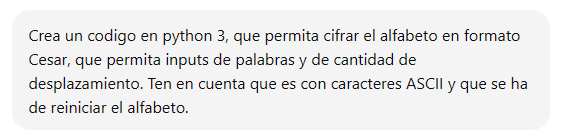
\includegraphics[width=8cm]{actividades/ac1/chatgpt_prompt.png}
        \caption{Prompt entregado a ChatGPT para la actividad 1.}
        \label{ac1 chatgpt prompt}
\end{figure}

La respuesta se muestra en la Figura \ref{ac1 chatgpt respuesta}. El código generado define una función (\verb|cifrado_cesar|) que recibe un texto y un número de desplazamiento. Dentro de la función, se recorren los caracteres del texto y, en caso de ser letras mayúsculas o minúsculas, se convierten a su valor ASCII mediante \verb|ord()|, se les aplica el desplazamiento con la operación módulo \% 26 para reiniciar el alfabeto al llegar al final, y luego se transforman nuevamente a caracteres con \verb|chr()|.

\begin{figure}[H]
    \centering
    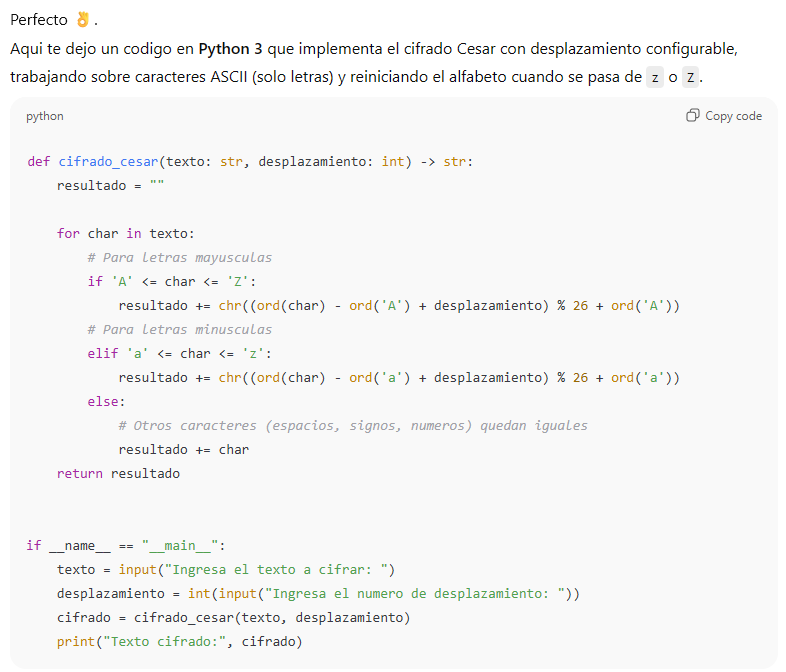
\includegraphics[width=10cm]{actividades/ac1/chatgpt_respuesta.png}
    \caption{Respuesta entregada por ChatGPT.}
    \label{ac1 chatgpt respuesta}
\end{figure}

El código entregado por ChatGPT cumple con la funcionalidad de aplicar el cifrado César de manera correcta. Sin embargo, se realizaron modificaciones para que los parámetros de entrada fueran recibidos directamente desde la terminal. Este cambio se hizo con el fin de seguir de forma más fiel el formato sugerido en la guía (ver sección \ref{actividad 1}). 
El resultado se puede ver en la Figura \ref{ac1 codigo modificado} o en el repositorio de GitHub como \href{https://github.com/BrunoTrone1/cripto_lab1/blob/main/algoritmo_cifrado.py}{algoritmo\_cifrado.py}.

\begin{figure}[H]
    \centering
    \begin{lstlisting}[language=Python]
import argparse

def cifrado_cesar(texto: str, desplazamiento: int) -> str:
    resultado = ""

    for char in texto:
        if 'A' <= char <= 'Z':
            resultado += chr((ord(char) - ord('A') + desplazamiento) % 26 + ord('A'))
        elif 'a' <= char <= 'z':
            resultado += chr((ord(char) - ord('a') + desplazamiento) % 26 + ord('a'))
        else:
            resultado += char
    return resultado

if __name__ == "__main__":
    parser = argparse.ArgumentParser(description="Cifrado Cesar")
    parser.add_argument("-t", "--texto", type=str, required=True, help="Texto a cifrar")
    parser.add_argument("-d", "--desplazamiento", type=int, required=True, help="Desplazamiento Cesar")
    args = parser.parse_args()

    cifrado = cifrado_cesar(args.texto, args.desplazamiento)
    print("Texto cifrado:", cifrado)
    \end{lstlisting}
    \caption{Código modificado para aceptar parámetros por terminal.}
    \label{ac1 codigo modificado}
\end{figure}  

El código implementa el cifrado César igual que código de ChatGPT, con la diferencia de que para las entradas se utiliza la biblioteca \verb|argparse|, la cual permite ingresar parámetros desde la línea de comandos. Con las banderas \verb|-t| para el texto y \verb|-d| para el desplazamiento.

La ejecución del programa resulta exitosa, como se muestra en la Figura \ref{ac1 codigo ejecutado}, donde puede observarse que la frase ingresada es cifrada de acuerdo con el número de desplazamientos especificado.

\begin{figure}[H]
    \centering
    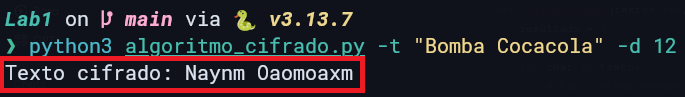
\includegraphics[width=9cm]{actividades/ac1/codigo_ejecutado.png}
    \caption{Código ejecutado, con la frase "Bomba Cocacola"\ cifrada "Naynm Oaomoaxm".}
    \label{ac1 codigo ejecutado}
\end{figure}

\subsection{Actividad 2}
\label{actividad 2 respuesta}
La actividad 2 consiste en enviar el mensaje cifrado en César mediante paquetes ICMP tipo Echo Request, de modo que cada carácter del mensaje se transmita en un paquete independiente. Para esto, se entregó un prompt a ChatGPT (Figura \ref{ac2 chatgpt prompt}), solicitando un programa en Python que permitiera dividir la palabra o frase y enviarla carácter por carácter usando ICMP.

\begin{figure}[H]
        \centering
        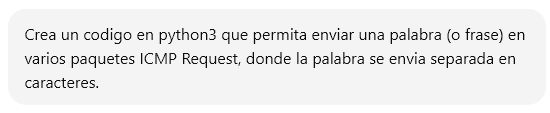
\includegraphics[width=8cm]{actividades/ac2/chatgpt_prompt.png}
        \caption{Prompt entregado a ChatGPT para la actividad 2.}
        \label{ac2 chatgpt prompt}
\end{figure}

 La respuesta generada se muestra en la Figura \ref{ac2 chatgpt respuesta}, como bloque de código en la Figura \ref{ac2 codigo} y disponible en GitHub como \href{https://github.com/BrunoTrone1/cripto_lab1/blob/main/modo_stealth.py}{modo\_stealth.py}. El código utiliza la librería Scapy para crear y enviar paquetes de red personalizados. Se importan las clases \verb|IP| y  \verb|ICMP| para construir las cabeceras de los paquetes, y la función \verb|send()| para transmitirlos. Además, se mantiene la biblioteca \verb|argparse| para recibir los parámetros de entrada: la dirección IP de destino con la bandera \verb|-d| y el mensaje con la bandera \verb|-m|.

\begin{figure}[H]
        \centering
        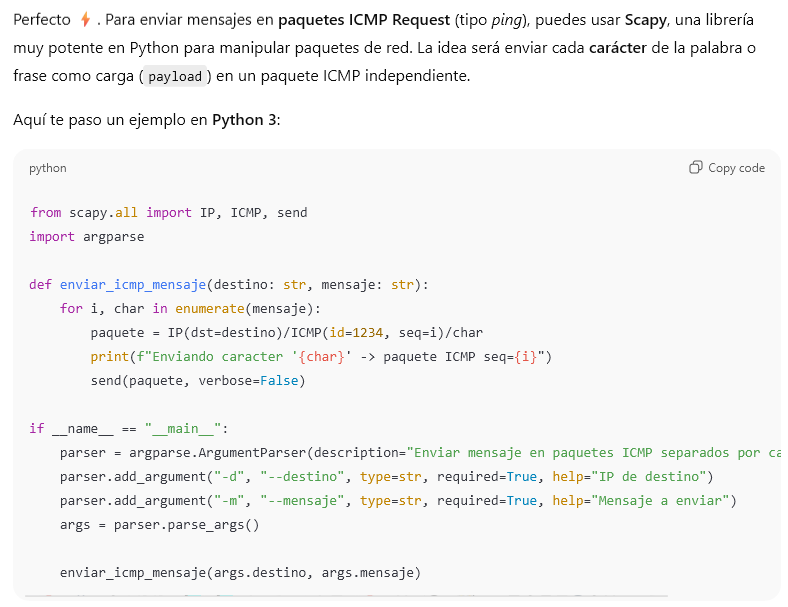
\includegraphics[width=14cm]{actividades/ac2/chatgpt_respuesta.png}
        \caption{Respuesta entregada por ChatGPT.}
        \label{ac2 chatgpt respuesta}
\end{figure}
\begin{figure}[H]
    \centering
    \begin{lstlisting}[language=Python]
from scapy.all import IP, ICMP, send
import argparse

def enviar_icmp_mensaje(destino: str, mensaje: str):
    for i, char in enumerate(mensaje):
        paquete = IP(dst=destino)/ICMP(id=1234, seq=i)/char
        print(f"Enviando caracter '{char}' -> paquete ICMP seq={i}")
        send(paquete, verbose=False)

if __name__ == "__main__":
    parser = argparse.ArgumentParser(description="Enviar mensaje en paquetes ICMP separados por caracteres")
    parser.add_argument("-d", "--destino", type=str, required=True, help="IP de destino")
    parser.add_argument("-m", "--mensaje", type=str, required=True, help="Mensaje a enviar")
    args = parser.parse_args()

    enviar_icmp_mensaje(args.destino, args.mensaje)
    \end{lstlisting}
    \caption{Código entregado por ChatGPT para enviar paquetes ICMP.}
    \label{ac2 codigo}
\end{figure}  

La ejecución del programa fue exitosa, como se observa en la Figura \ref{ac2 codigo ejecutado}, donde se envió la frase "Naynm Oaomoaxm", transmitiendo cada carácter en un paquete ICMP independiente.

\begin{figure}[H]
        \centering
        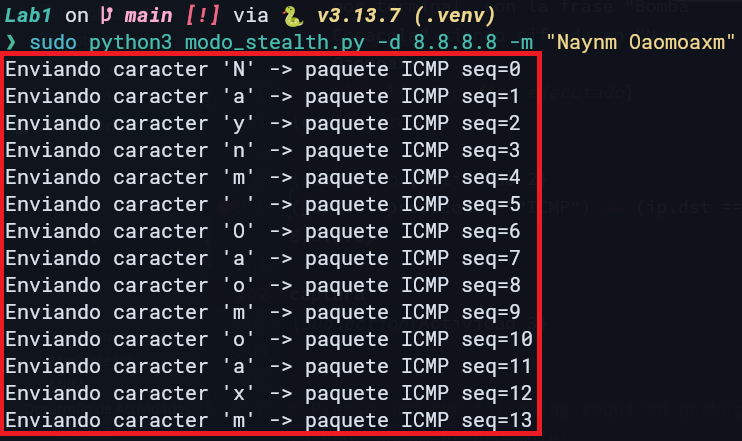
\includegraphics[width=15cm]{actividades/ac2/codigo_ejecutado.png}
        \caption{Resultado del código ejecutado por terminal, con la frase "Naynm Oaomoaxm" \ enviada en paquetes ICMP.}
        \label{ac2 codigo ejecutado}
\end{figure}

La correcta segmentación y envío del mensaje se puede verificar mediante Wireshark (disponible en el GitHub como \href{https://github.com/BrunoTrone1/cripto_lab1/blob/main/captura.pcap}{captura.pcap}), aplicando filtros por protocolo ICMP y destino 8.8.8.8 (\verb|(_ws.col.protocol == "ICMP") && (ip.dst == 8.8.8.8)|), como se muestra en la Figura \ref{ac2 captura wireshark}.

\begin{figure}[H]
        \centering
        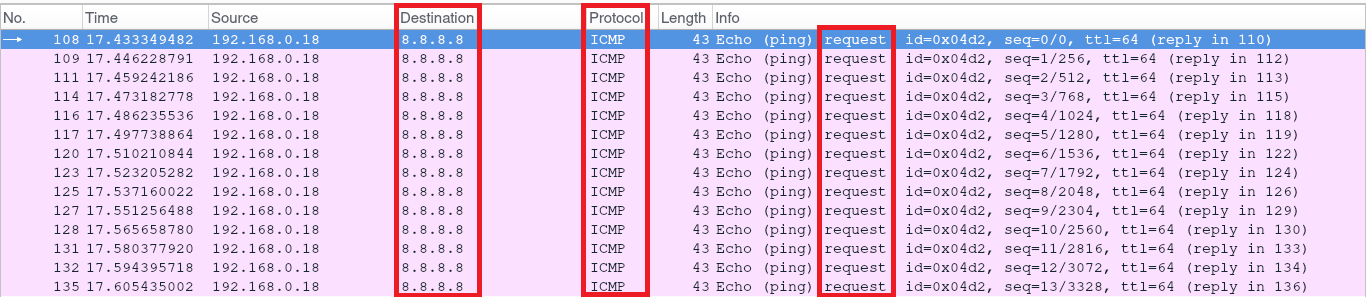
\includegraphics[width=\linewidth]{actividades/ac2/captura_wireshark.png}
        \caption{Captura de paquetes en Wireshark, con el filtro para protocolo ICMP y destino 8.8.8.8.}
        \label{ac2 captura wireshark}
\end{figure}

Cada paquete puede inspeccionarse individualmente; la Figura \ref{ac2 caracter 0} muestra el primer carácter "N" transmitido en un paquete ICMP, evidenciando que el campo de datos contiene correctamente el carácter enviado (por temas de espacio, solo se muestra el primer carácter, los demás están disponibles en GitHub dentro de la carpeta \href{https://github.com/BrunoTrone1/cripto_lab1/tree/main/actividades/ac2}{actividades/ac2}).

\begin{figure}[H]
        \centering
        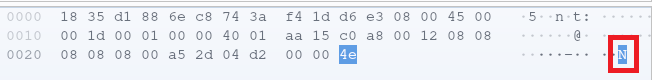
\includegraphics[width=\linewidth]{actividades/ac2/caracter_0.png}
        \caption{Captura del primer carácter "N" \ enviado mediante ICMP por Wireshark.}
        \label{ac2 caracter 0}
\end{figure}

\subsection{Actividad 3}
\label{actividad 3 respuesta}
La actividad 3 consiste en descifrar mensajes enviados carácter por carácter mediante paquetes ICMP, aplicando el cifrado César sin conocer de antemano el número de desplazamientos. Para esto, se entregó un prompt a ChatGPT (Figura \ref{ac3 prompt chatgpt}), solicitando un programa en Python que pudiera procesar una captura de Wireshark (\verb|.pcap|), reconstruir el mensaje y determinar automáticamente el desplazamiento más probable usando un diccionario de palabras en español.

\begin{figure}[H]
        \centering
        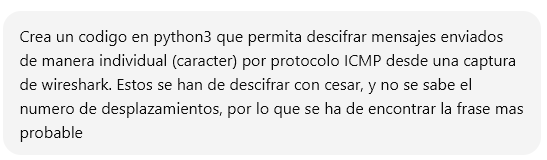
\includegraphics[width=8cm]{actividades/ac3/chatgpt_prompt.png}
        \caption{Prompt entregado a ChatGPT para la actividad 3}
        \label{ac3 prompt chatgpt}
\end{figure}

La respuesta generada se muestra en la Figura \ref{ac3 respuesta chatgpt}. El código proporcionado utiliza la librería Scapy para leer los paquetes ICMP desde un archivo \verb|.pcap| y extraer los caracteres del payload. Cada carácter del mensaje original enviado en paquetes ICMP tipo Echo Request (\verb|type == 8|) se concatena para formar la cadena completa recibida.

Para descifrar el mensaje, se implementa la función \verb|descifrado_cesar|, que aplica un desplazamiento inverso a cada letra, considerando mayúsculas y minúsculas y manteniendo los caracteres no alfabéticos sin cambios. Dado que no se conoce el desplazamiento, la función \verb|obtener_mensaje_mas_probable| prueba todos los valores posibles (0–25) y utiliza la librería \verb|pyspellchecker| (en este caso usada como diccionario en español) para determinar cuál produce la mayor cantidad de palabras válidas, seleccionando así la frase más probable.

\begin{figure}[H]
        \centering
        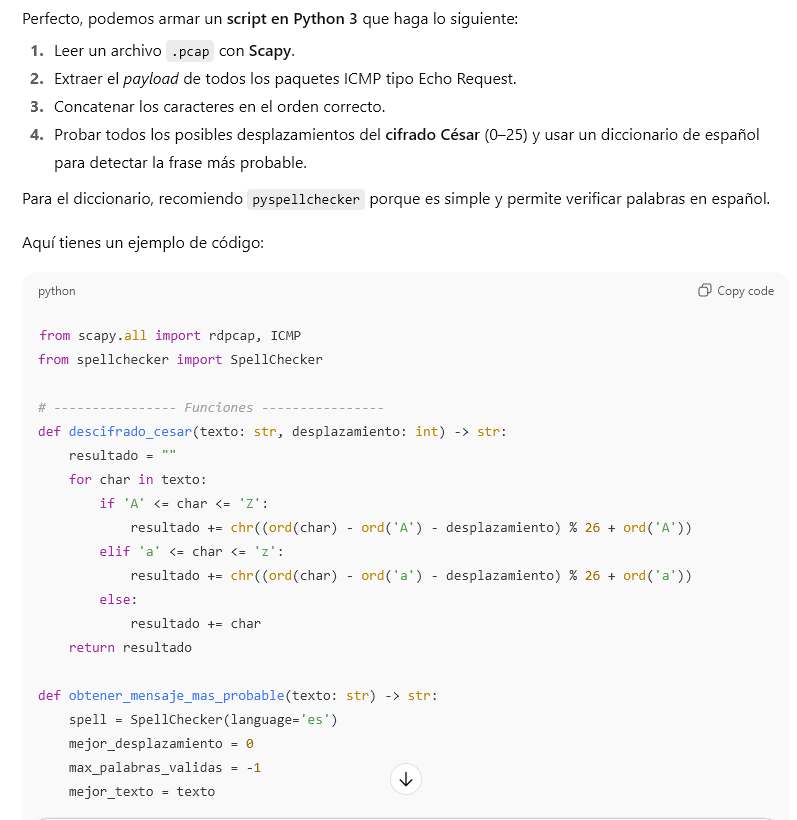
\includegraphics[width=15cm]{actividades/ac3/chatgpt_respuesta.png}
        \caption{Respuesta entregada por ChatGPT.}
        \label{ac3 respuesta chatgpt}
\end{figure}

El código entregado por ChatGPT se mantiene en su lógica y funcionamiento, con la única modificación de que se incorporó la librería \verb|argparse| para permitir ingresar desde la terminal el nombre del archivo \verb|.pcap| que se desea procesar. Esto hace que el script sea más flexible y se pueda ejecutar con diferentes capturas sin necesidad de modificar el código internamente. El resultado se puede observar en la Figura \ref{ac3 codigo} y en el repositorio de GitHub como \href{https://github.com/BrunoTrone1/cripto_lab1/blob/main/MitM.py}{MitM.py}.

\begin{figure}[H]
    \centering
    \begin{lstlisting}[language=Python]
from scapy.all import rdpcap, ICMP
from spellchecker import SpellChecker
import argparse

def descifrado_cesar(texto: str, desplazamiento: int) -> str:
    resultado = ""
    for char in texto:
        if 'A' <= char <= 'Z':
            resultado += chr((ord(char) - ord('A') - desplazamiento) % 26 + ord('A'))
        elif 'a' <= char <= 'z':
            resultado += chr((ord(char) - ord('a') - desplazamiento) % 26 + ord('a'))
        else:
            resultado += char
    return resultado

def obtener_mensaje_mas_probable(texto: str) -> str:
    spell = SpellChecker(language='es')
    mejor_desplazamiento = 0
    max_palabras_validas = -1
    mejor_texto = texto

    for d in range(26):
        descifrado = descifrado_cesar(texto, d)
        palabras = descifrado.split()
        validas = sum(1 for w in palabras if w.lower() in spell)
        if validas > max_palabras_validas:
            max_palabras_validas = validas
            mejor_desplazamiento = d
            mejor_texto = descifrado

    print(f"Mejor desplazamiento encontrado: {mejor_desplazamiento}")
    return mejor_texto
...
    \end{lstlisting}
    \caption{Extracto del código modificado para descifrar y aceptar archivos por terminal.}
    \label{ac3 codigo}
\end{figure}  

La ejecución del código fue exitosa, como se observa en la Figura \ref{ac3 codigo ejecutado}. En este ejemplo, se procesó el mensaje recibido "Naynm Oaomoaxm", se determinó el desplazamiento más probable y se recuperó correctamente la frase original "Bomba Cocacola". Esto confirma que el programa es capaz de reconstruir mensajes enviados carácter por carácter mediante ICMP y descifrarlos automáticamente.

\begin{figure}[H]
        \centering
        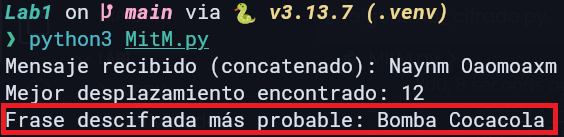
\includegraphics[width=9cm]{actividades/ac3/codigo_ejecutado.png}
        \caption{Resultado del código ejecutado por terminal, con el mensaje recibido "Naynm Oaomoaxm"\ , el mejor desplazamiento y la frase encontrada "Bomba Cocacola".}
        \label{ac3 codigo ejecutado}
\end{figure}

Se eligió ChatGPT como IA generativa por experiencias previas con Python, donde demostró buen rendimiento y generó código claro y funcional. Solo fue necesario ajustar la entrada por terminal con \verb|argparse| para mayor flexibilidad, sin problemas significativos durante la generación y ejecución del código.

\section*{Conclusiones y comentarios}
\label{conclusiones}
El desarrollo de este laboratorio permitió aplicar de manera práctica conceptos fundamentales de seguridad informática, en particular el uso de cifrado clásico, el encubrimiento de información en tráfico legítimo y la recuperación de mensajes mediante técnicas de análisis. En la primera actividad se implementó el algoritmo César, reforzando el entendimiento de cómo los métodos de sustitución desplazan el alfabeto y la importancia de parametrizar adecuadamente un programa. Posteriormente, en la segunda actividad, se puso en práctica el envío de datos encubiertos en paquetes ICMP, evidenciando la facilidad con la que información sensible puede ser transmitida sin generar alertas aparentes. Finalmente, en la tercera actividad se desarrolló un proceso de descifrado y análisis automático, que no solo permitió recuperar el mensaje original, sino también comprobar la vulnerabilidad de estos métodos frente a ataques de intermediario.

En conjunto, este laboratorio entregó una visión integral del ciclo completo de ocultación, transmisión y detección de información en redes, demostrando tanto la creatividad que puede emplearse para evadir sistemas de inspección como la importancia de contar con herramientas de auditoría robustas. Asimismo, se adquirió experiencia en el uso de bibliotecas de Python orientadas a redes y procesamiento de datos, y se reforzó la capacidad de evaluar críticamente la seguridad de un sistema a través de pruebas de concepto controladas. Además, se demostró que utilizar ChatGPT como IA generativa, sumado al conocimiento previo, constituye una herramienta eficiente y valiosa para apoyar el desarrollo de soluciones en este tipo de trabajos.

\end{document}
